\label{ch:compressible}

\begin{quote}
\noindent {\em These notes describe how to do a piecewise linear or
  piecewise parabolic method for the Euler equations.  These are the
  basis for some of the most popular methods in astrophysics.}
\end{quote}

%-----------------------------------------------------------------------------
\section{Euler equation properties}

The Euler equations in one dimension appear as:
\begin{align}
\frac{\partial \rho}{\partial t} + 
    \frac{\partial (\rho u)}{\partial x} &= 0 \\
%
\frac{\partial(\rho u)}{\partial t} +
    \frac{\partial (\rho uu + p)}{\partial x} &= 0 \\
%
\frac{\partial(\rho E)}{\partial t} + 
    \frac{\partial(\rho u E + u p)}{\partial x} &= 0
\end{align}
These represent conservation of mass, momentum, and energy.  Here $\rho$ is the
density, $u$ is the one-dimensional velocity, $p$ is the pressure, and $E$
is the total energy / mass, and can be expressed in terms of the
specific internal energy and kinetic energy as:
\begin{equation}
E = e + \frac{1}{2} u^2
\end{equation}
The equations are closed with the addition of an equation of state.  A common
choice is the gamma-law EOS:
\begin{equation}
p = \rho e(\gamma - 1)
\end{equation}
where $\gamma$ is the ratio of specific heats for the gas/fluid (for
an ideal, monatomic gas, $\gamma = 5/3$), but any relation of the form
$p = p(\rho, e)$ will work.  

One thing that we can notice immediately is that there is no need for
temperature in this equation set, although often, when source terms
are present, we will need to obtain temperature from the equation of
state.

In this form, the equations are said to be in {\em conservative form},
i.e.\ they can be written as:
\begin{equation}
U_t + \left [F(U) \right ]_x = 0
\end{equation}
with
\begin{equation}
U = \left ( \begin{array}{c} \rho \\ \rho u \\ \rho E \end{array} \right )
%
\qquad
%
F(U) = \left ( \begin{array}{c} \rho u \\ \rho uu + p \\ \rho u E + up \end{array} \right )
\end{equation}
%
We can write this in {\em quasi-linear} form by first expressing the flux
vector in terms of the conserved variables directly.  Taking $u_1 =
\rho, u_2 = \rho u, u_3 = \rho E$, we have
\begin{equation}
F(U) = \left ( \begin{array}{c} 
      u_2 \\
      \frac{u_2^2}{u_1} \left (1 - \frac{\hat{\gamma}}{2} \right ) + u_3 \hat{\gamma} \\
      \frac{u_3 u_2}{u_1}(1 + \hat{\gamma}) - \frac{1}{2} \frac{u_2^3}{u_1^2} \hat{\gamma} \end{array} \right )
\end{equation}
where $\hat{\gamma} = \gamma - 1$, and $p = \rho e \hat{\gamma} = (\rho E - \rho u^2/2)\hat{\gamma}$.  The Jacobian of this flux vector is $A = \partial F/\partial U$:
\begin{equation}
A(U) = \left ( \begin{array}{ccc} 
   0  & 1 & 0 \\
   -\frac{1}{2}u^2(3 -\gamma) & u (3 -\gamma) & \gamma - 1 \\
   \frac{1}{2}(\gamma -2)u^3 - \frac{uc^2}{\gamma -1} &
       \frac{3-2\gamma}{2} u^2 + \frac{c^2}{\gamma -1} & u \gamma
  \end{array} \right )
\end{equation}
where the speed of sound is $c = \sqrt{\gamma p/\rho}$.   With this, our
system can be written as:
\begin{equation}
U_t + A(U) U_x = 0
\end{equation}
This matrix is quite complex and difficult to work with.  The
eigenvectors of this matrix can be found in a variety of sources
(e.g. \cite{toro:1997,athena}).


An alternate way to express these equations is using the {\em
  primitive variables}: $\rho, u, p$.
\begin{exercise}[Primitive variable form of the Euler equations]
{Show that the Euler equations in primitive form can
  be written as
\begin{equation}
q_t + A(q) q_x = 0
\end{equation}
where
\begin{equation}
q = \left ( \begin{array}{c} \rho \\ u \\ p \end{array} \right )
%
\qquad
A(q) = \left ( \begin{array}{ccc} u  & \rho     & 0 \\
                                  0  &  u       & 1/\rho \\
                                  0  & \gamma p & u \end{array} \right )
\label{eq:primitivesystem}
\end{equation}
}
\end{exercise}
%
The eigenvalues of $A$ can be found via $| A - \lambda I | = 0$,
where $|\ldots|$ indicates the determinant and $\lambda$ are the eigenvalues.
\begin{exercise}[The eigenvalues of the Euler system]
{
Show that the eigenvalues of $A$ are $\lambda^\evm = u -c$, $\lambda^\evz = u$, $\lambda^\evp = u+c$.
}
\end{exercise}
Note that both the conserved Jacobian matrix, $A(U)$, and the
primitive variable matrix, $A(q)$, have the same eigenvalues---as
expected, since they represent the same physics.  Also note that in
Eq.~\ref{eq:primitivesystem}, we used the algebraic gamma-law equation
of state to replace $e$ with $p$, however, for a general equation of state,
we can get the appropriate expression by writing $p = p(\rho, s)$:
\begin{equation}
\frac{Dp}{Dt} = \left . \frac{\partial p}{\partial \rho} \right |_s
     \frac{D\rho}{Dt} +
     \left . \frac{\partial p}{\partial s} \right |_\rho
     \cancelto{0}{\frac{Ds}{Dt}}
\end{equation}
where $Ds/Dt$ is $0$ when no entropy sources are present.  Recognizing
that $\Gamma_1 \equiv \partial \log p/\partial \log \rho |_s$, we have:
\begin{equation}
\frac{\partial p}{\partial t} + u \frac{\partial p}{\partial x} 
  + \Gamma_1 p \frac{\partial u}{\partial x} = 0  \label{eq:euler:pgeneral}
\end{equation}
as the generalization of the pressure equation.

We'll use the symbols $\{-,\circ,+\}$ to denote the eigenvalues and their
corresponding eigenvectors thoughout these notes.
These eigenvalues are the speeds at which information propagates through
the fluid.
Since the eigenvalues are real, this system (the Euler equations) is said
to be {\em hyperbolic}.  Additionally, since $A = A(q)$, the system is
said to be {\em quasi-linear}.  
%
The right and left eigenvectors can be found via:
\begin{equation}
A \, r^\enu = \lambda^\enu r^\enu \; ;
\qquad
l^\enu \, A  = \lambda^\enu l^\enu
\end{equation}
where $\nu = \{-,\circ,+\}$ corresponding to the three waves, and 
there is one right and one left eigenvector for each of the eigenvalues.
%
\begin{exercise}[Eigenvectors of the Euler system]
{
Show that the right eigenvectors are:
\begin{equation}
r^\evm = \left ( \begin{array}{c} 1 \\ -c/\rho \\ c^2 \end{array} \right )
%
\qquad
r^\evz = \left ( \begin{array}{c} 1 \\ 0 \\ 0  \end{array} \right )
%
\qquad
r^\evp = \left ( \begin{array}{c} 1 \\ c/\rho \\ c^2 \end{array} \right )
\end{equation}
and the left eigenvectors are:
\begin{align}
l^\evm &= \left ( \begin{array}{ccc} 0 & -\frac{\rho}{2c} & \frac{1}{2c^2} 
                  \end{array} \right ) \\
%
\qquad
l^\evz &= \left ( \begin{array}{ccc} 1 & 0 & -\frac{1}{c^2}  \end{array} \right ) \\
%
\qquad
l^\evp &= \left ( \begin{array}{ccc} 0 & \phantom{+}\frac{\rho}{2c} & \frac{1}{2c^2} \end{array} \right )
\end{align}
Note that in general, there can be an arbitrary constant in front of each
eigenvector.  Here they are normalized such that 
$l^{(i)} \cdot r^{(j)} = \delta_{ij}$.
}
\end{exercise}

A final form of the equations is called the {\em characteristic form}.  Here,
we wish to diagonalize the matrix $A$.  We take the matrix $R$ to be the
matrix of right eigenvectors, $R = (r^\evm | r^\evz | r^\evp )$, and $L$
is the corresponding matrix of left eigenvectors:
\begin{equation}
L = \left ( \begin{array}{c} l^\evm \\              
                             \hdashline 
                             l^\evz \\
                             \hdashline 
                             l^\evp \end{array} \right )
\end{equation}
Note that $L\, R = I = R\, L$, and
$L = R^{-1}$.
\begin{exercise}[Characteristic form of the Euler equations]
{
Show that $\Lambda = L A R$ is a diagonal matrix with the diagonal elements
simply the 3 eigenvalues we found above:
\begin{equation}
\Lambda = 
   \left ( \begin{array}{ccc}
             \lambda^\evm &              & \\
                          & \lambda^\evz & \\
                          &              & \lambda^\evp \end{array} \right )
\end{equation}
}
\end{exercise}
Defining $dw = L dq$, we can write our system as:
\begin{equation}
w_t + \Lambda w_x = 0
\end{equation}
Here, the $w$ are the characteristic variables.  Note that we cannot
in general integrate $dw = L dq$ to write down the characteristic
quantities.  Since $\Lambda$ is diagonal, this system is a set of
decoupled advection-like equations.  If the system were linear, then the
solution to each would simply be to advect the quantity $w^\enu$ at
the wave speed $\lambda^\enu$.

Imagine initial conditions consisting of a jump in the primitive
variables, $\Delta q$.  The corresponding characteristic variables are
$\Delta w \sim L \Delta q$ (where the $\sim$ accounts for the fact
that in a nonlinear system, $L = L(q)$).  The characteristic form
of the equations says that each of the waves will carry with it
a jump in $w$.  Since $dq = L^{-1}dw = R dw$, the jump
in the primitive variable across each wave is proportional to the
right-eigenvector associated with that wave.  So, for example, since
$r^\evz$ is only non-zero for the density element, this then means
that only density jumps across the $\lambda^\evz = u$ wave---pressure
and velocity are constant across this wave (see for example,
Toro~\cite{toro:1997}, Ch.\ 2, 3 or LeVeque~\cite{leveque:2002} for a
thorough discussion).  Figure~\ref{fig:sod} shows the three waves
emanating from an initial discontinuity.

\begin{figure}
\centering
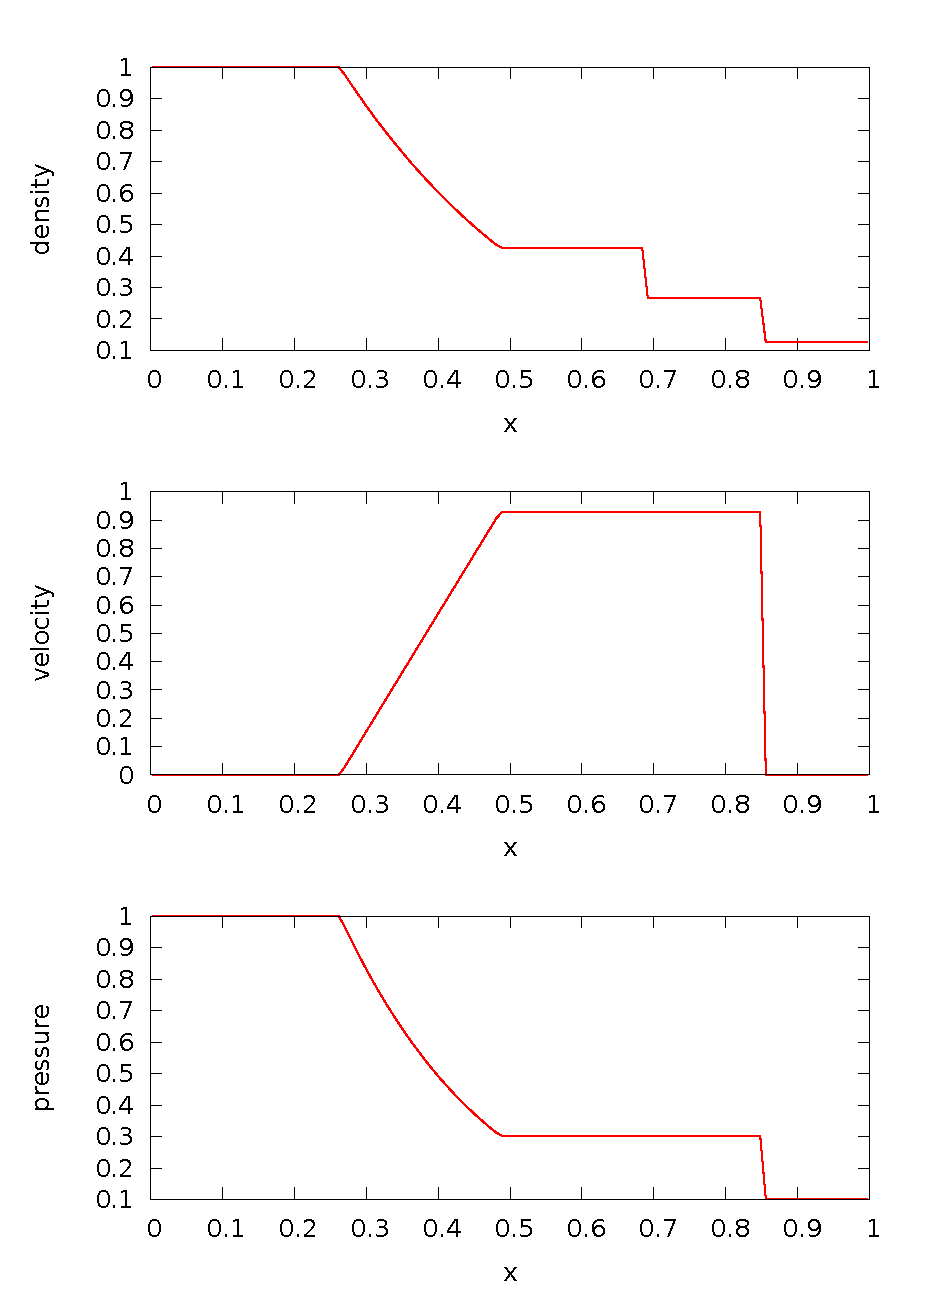
\includegraphics[width=0.85\linewidth]{sod}
\caption[The Sod problem.]{\label{fig:sod} Evolution following from an initial
  discontinuity at $x = 0.5$.  These particular conditions are called
  the {\em Sod problem}, and in general, a setup with two states
  separated by a discontinuity is called a shock-tube problem.  Here
  we see the three waves propagating away from the initial
  discontinuity.  The left ($u-c$) wave is a rarefaction, the middle
  ($u$) is the contact discontinuity, and the right ($u+c$) is a
  shock. Note that all 3 primitive variables jump across the left and
  right waves, but only the density jumps across the middle wave.
  This reflects the right eigenvectors.  Also note that no waves have
  reached the far left and far right yet, the conditions there are the
  same as the initial conditions.}
\end{figure}


%-----------------------------------------------------------------------------
\section{Other Thermodynamic Equations}

At times we will want to use alternate forms of the energy equation.  The
internal energy is governed by the first law of thermodynamics.  In the
absense of any heat sources, we have:
\begin{equation}
dq = 0 = de + pd(1/\rho)
\end{equation}
where $e$ is the specific internal energy.
Applying this to a Lagrangian fluid element, we have:
\begin{align}
\frac{De}{Dt} + p \frac{D(1/\rho)}{Dt} &= 0 \\
\frac{De}{Dt} - \frac{1}{\rho^2} \frac{D\rho}{Dt} &= 0 \\
\rho \frac{De}{Dt} + p \nabla \cdot U &= 0
\end{align}
where we used the continuity equation in the last step to eliminate
$D\rho/Dt$.  This can be rewritten by adding $e \times$ the continuity
equation to give:
\begin{equation}
\frac{\partial (\rho e)}{\partial t} + \nabla \cdot (\rho U e) + p \nabla \cdot U = 0 \label{eq:euler:econs}
\end{equation}


%-----------------------------------------------------------------------------
\section{Reconstruction of interface states}

\label{sec:onedrecon}

We will solve the Euler equations using a high-order {\em Godunov
  method}---a finite volume method whereby the fluxes through the
interfaces are computed by solving the Riemann problem for our system.
The finite-volume update for our system appears as:
\begin{equation}
U^{n+1}_i = U^n_i + \frac{\Delta t}{\Delta x} \left ( F_{i-1/2}^{n+1/2} - F_{i+1/2}^{n+1/2} \right )
\end{equation}
This says that each of the conserved quantities in $U$ change only due
to the flux of that quantity through the boundary of the cell.

Instead of approximating the flux itself on the interface, we find an
approximation to the state on the interface, $U_{i-1/2}^{n+1/2}$ and
$U_{i+1/2}^{n+1/2}$ and use this with the flux function to define the
flux through the interface:
\begin{align}
F_{i-1/2}^{n+1/2} &= F(U_{i-1/2}^{n+1/2}) \\
F_{i+1/2}^{n+1/2} &= F(U_{i+1/2}^{n+1/2})
\end{align}
To find this interface state, we predict left and right states at each
interface (centered in time), which are the input to the Riemann
solver.  The Riemann solver will then look at the characteristic wave
structure and determine the fluid state on the interface, which is
then used to compute the flux.  This is illustrated in
Figure~\ref{fig:riemann}.  

Finally, although we use the conserved variables for the final update,
in constructing the interface states it is often easier to work with
the primitive variables.  These have a simpler characteristic
structure.  The interface states in terms of the primitive variables
can be converted into the interface states of the conserved variables
through a simple algebraic transformation, 
\begin{equation}
U_{i+1/2,L}^{n+1/2} = U(q_{i+1/2,L}^{n+1/2})
\end{equation}

\begin{figure}[t]
\centering
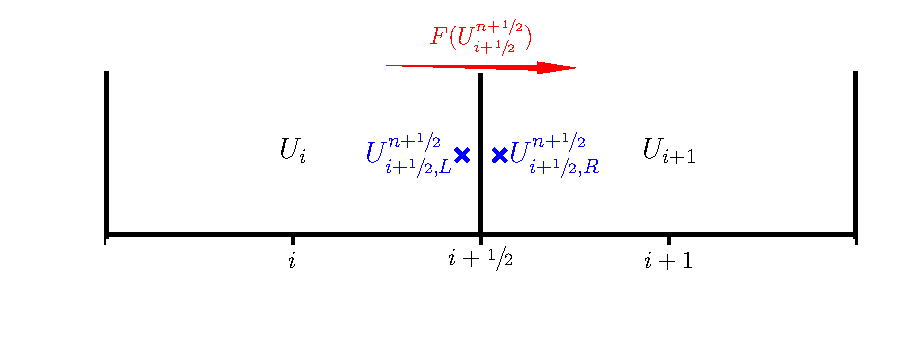
\includegraphics[width=\linewidth]{riemann_comp}
\caption[The left and right states for the Riemann
  problem.]{\label{fig:riemann} The left and right states at interface
  $i+1/2$.  The arrow indicates the flux through the interface, as
  computed by the Riemann solver using these states as input.}
\end{figure}

Constructing these interface states requires reconstructing the
cell-average data with a piecewise constant, linear, or parabolic
polynomial and doing characteristic tracing to see how much of each
characteristic quantity comes to the interface over the timestep.  The
jump in the primitive variables is projected into the characteristic
variables, and only jumps moving toward the interface are included in
our reconstruction.  We look at several methods below that build off
of these ideas below.

\subsection{Piecewise constant}

The simplest possible reconstruction of the data is piecewise constant.
This is what was done in the original Godunov method.  For the interface
marked by $i+1/2$, the left and right states on the interface are simply:
\begin{align}
U_{i+1/2,L} &= U_i \\
U_{i+1/2,R} &= U_{i+1}
\end{align}
This does not take into account in any way how the state $U$ may be changing
through the cell.  As a result, it is first-order accurate in space, and since
no attempt was made to center it in time, it is first-order accurate in time.

\subsection{Piecewise linear}

For higher-order reconstruction, we first convert from the conserved
variables, $U$, to the primitive variables, $q$.  These have a simpler
characteristic structure, making them easier to work with.  Here we
consider piecewise linear reconstruction---the cell average data is
approximated by a line with non-zero slope within each cell.
Figure~\ref{fig:plm} shows the piecewise linear reconstruction of some
data.

\begin{figure}[t]
\centering
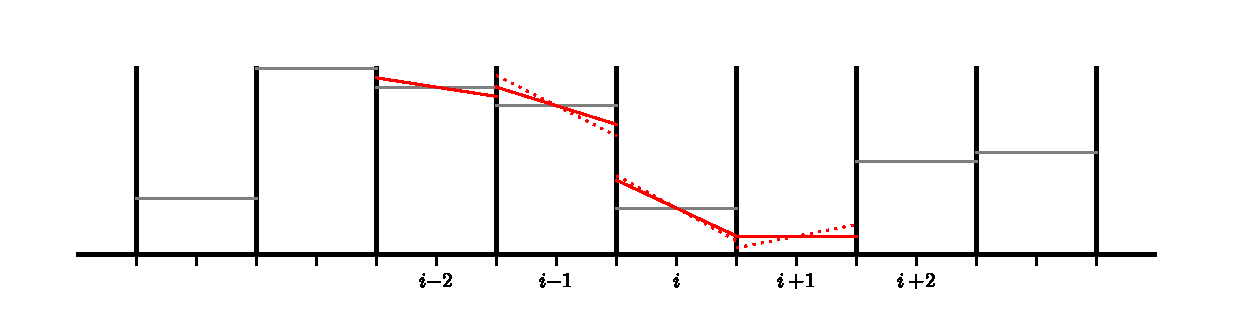
\includegraphics[width=\linewidth]{piecewise-linear}
\caption[Piecewise linear reconstruction of cell average
  data.]{\label{fig:plm} Piecewise linear reconstruction of the cell
  averages.  The dotted line shows the unlimited center-difference
  slopes and the solid line shows the limited slopes.}
\end{figure}

Consider constructing the left state at the interface $i+1/2$ (see
Figure~\ref{fig:riemann}).  Just like for the advection equation, we
do a Taylor expansion through $\Delta x/2$ to bring us to the
interface, and $\Delta t/2$ to bring us to the midpoint in time.
Starting with $q_i$, the cell-centered primitive variable, expanding
to the right interface (to create the left state there) gives:
\begin{align}
q_{i+1/2,L}^{n+1/2} &= q_i^n + 
    \left . \frac{\Delta x}{2} \frac{\partial q}{\partial x} \right |_i +
    \frac{\Delta t}{2} \underbrace{\left .\frac{\partial q}{\partial t} \right |_i}_{= -A \partial q / \partial x} + \ldots \\
&= q_i^n + \frac{\Delta x}{2} \left . \frac{\partial q}{\partial x} \right |_i
          - \frac{\Delta t}{2} \left ( A \frac{\partial q}{\partial x} \right )_i\\
&= q_i^n + \frac{1}{2} \left [ 1 - \frac{\Delta t}{\Delta x} A_i \right ] \Delta q_i \label{eq:taylorstate}
\end{align}
where $\Delta q_i$ is the reconstructed slope of the primitive
variable in that cell (similar to how we compute it for the advection
equation).  We note that the terms truncated in the first line are
$O(\Delta x^2)$ and $O(\Delta t^2)$, so our method will be second-order
accurate in space and time.

As with the advection equation, we limit the slope such that no new minima
or maxima are introduced.  Any of the slope limiters used for linear advection
apply here as well.  We represent the limited slope as $\overline{\Delta q}_i$.

We can decompose $A \Delta q$ in terms of the left and right
eigenvectors and sum over all the waves that move {\em toward} the
interface.  First, we recognize that $A = R \Lambda L$ and recognizing
that the `$1$'
in Eq.~\ref{eq:taylorstate} is the identity, $I = LR$, we rewrite this
expression as:
\begin{equation}
q_{i+1/2,L}^{n+1/2} = q_i^n + 
     \frac{1}{2} \left [ RL - \frac{\Delta t}{\Delta x} R\Lambda L \right ]_i \overline{\Delta q}_i
\end{equation}
We see the common factor of $L \Delta q$.  We now write this back in
component form.  Consider:
\begin{equation}
\renewcommand{\arraystretch}{1.5}
R\Lambda L \overline{\Delta q} =
   \left ( \begin{array}{c:c:c}
             r_1^\evm & r_1^\evz & r_1^\evp \\
             r_2^\evm & r_2^\evz & r_2^\evp \\
             r_3^\evm & r_3^\evz & r_3^\evp \end{array} \right )
   \left ( \begin{array}{ccc}
             \lambda^\evm &              & \\
                          & \lambda^\evz & \\
                          &              & \lambda^\evp \end{array} \right )
   \left ( \begin{array}{ccc}
             l_1^\evm & l_2^\evm & l_3^\evm \\
             \hdashline 
             l_1^\evz & l_2^\evz & l_3^\evz \\
             \hdashline
             l_1^\evp & l_2^\evp & l_3^\evp \end{array} \right )
   \left ( \begin{array}{c}
            \overline{\Delta \rho} \\
            \overline{\Delta u} \\
            \overline{\Delta p} \end{array} \right )
\renewcommand{\arraystretch}{1.0}
\end{equation}
Starting with $L \overline{\Delta q}$, which is a vector with each component
the dot-product of a left eigenvalue with $\overline{\Delta q}$, we have
\begin{equation}
\renewcommand{\arraystretch}{1.5}
R\Lambda L \overline{\Delta q} =
   \left ( \begin{array}{c:c:c}
             r_1^\evm & r_1^\evz & r_1^\evp \\
             r_2^\evm & r_2^\evz & r_2^\evp \\
             r_3^\evm & r_3^\evz & r_3^\evp \end{array} \right )
   \left ( \begin{array}{ccc}
             \lambda^\evm &              & \\
                          & \lambda^\evz & \\
                          &              & \lambda^\evp \end{array} \right )
   \left ( \begin{array}{c}
            l^\evm \cdot \overline{\Delta q} \\
            l^\evz \cdot \overline{\Delta q} \\
            l^\evp \cdot \overline{\Delta q} \end{array} \right )
\renewcommand{\arraystretch}{1.0}
\end{equation}
Next we see that multiplying this vector by $\Lambda$ simply puts the
eigenvalue with its respective eigenvector in the resulting column vector:
\begin{equation}
\renewcommand{\arraystretch}{1.5}
R\Lambda L \overline{\Delta q} =
   \left ( \begin{array}{c:c:c}
             r_1^\evm & r_1^\evz & r_1^\evp \\
             r_2^\evm & r_2^\evz & r_2^\evp \\
             r_3^\evm & r_3^\evz & r_3^\evp \end{array} \right )
   \left ( \begin{array}{c}
            \lambda^\evm \, l^\evm \cdot \overline{\Delta q} \\
            \lambda^\evz \, l^\evz \cdot \overline{\Delta q} \\
            \lambda^\evp \, l^\evp \cdot \overline{\Delta q} \end{array} \right )
\renewcommand{\arraystretch}{1.0}
\end{equation}
Finally, the last multiply results in a column vector:
\begin{equation}
\renewcommand{\arraystretch}{1.5}
R\Lambda L \overline{\Delta q} =
   \left ( \begin{array}{c}
            r_1^\evm \, \lambda^\evm \, l^\evm \cdot \overline{\Delta q} +
            r_1^\evz \, \lambda^\evz \, l^\evz \cdot \overline{\Delta q} +
            r_1^\evp \, \lambda^\evp \, l^\evp \cdot \overline{\Delta q} \\
%
            r_2^\evm \, \lambda^\evm \, l^\evm \cdot \overline{\Delta q} +
            r_2^\evz \, \lambda^\evz \, l^\evz \cdot \overline{\Delta q} +
            r_2^\evp \, \lambda^\evp \, l^\evp \cdot \overline{\Delta q} \\
%
            r_3^\evm \, \lambda^\evm \, l^\evm \cdot \overline{\Delta q} +
            r_3^\evz \, \lambda^\evz \, l^\evz \cdot \overline{\Delta q} +
            r_3^\evp \, \lambda^\evp \, l^\evp \cdot \overline{\Delta q} \\
   \end{array} \right )
\renewcommand{\arraystretch}{1.0}
\end{equation}
We can rewrite this compactly as:
\begin{equation}
\sum_\nu \lambda^{(\nu)} (l^{(\nu)} \cdot \overline{\Delta q}) r^{(\nu)}
\end{equation}
where we use $\nu$ to indicate which wave we are summing over.  A similar 
expansion is used for $RL \overline{\Delta q}$.  In fact, any vector
can be decomposed in this fashion:
\begin{equation}
\chi = I \chi = R L \chi = \sum_\nu (l^\enu \cdot \chi) r^\enu
\end{equation}
And then it is easy to see that the above manipulations for $A \Delta q$
can be expressed as:
\begin{equation}
A \Delta q =  A \sum_\nu (l^\enu \cdot \overline{\Delta q}) r^\enu = \sum_\nu (l^\enu \cdot \overline{\Delta q}) A r^\enu = \sum_\nu (l^\enu \cdot \overline{\Delta q}) \lambda^\enu r^\enu
\end{equation} 
where we used $A r^\enu = \lambda^\enu r^\enu$.  The quantity $(l^\enu
\cdot \overline{\Delta q})$ that shows up here is the projection of
the vector $\overline{\Delta q}$ into the characteristic variable
carried by wave $\nu$.  This sum shows, as discussed earlier, that each wave
carries a jump in the characteristic variable, with the jump in the primitive
variables proportion to the right eigenvector, $r^\enu$.

The resulting vector
for the left state is:
\begin{equation}
q_{i+1/2,L}^{n+1/2} = q_i^n + \frac{1}{2} \sum_{\nu; \lambda^{(\nu)} \ge 0} 
  \left [ 1 - \frac{\Delta t}{\Delta x} \lambda_i^{(\nu)} \right ] (l_i^{(\nu)} \cdot \overline{\Delta q}_i) r_i^{(\nu)} 
\end{equation}
Note that we make a slight change here, and only include a term in the sum if
its wave is moving toward the interface ($\lambda^\enu \ge 0$).  The quantity
$\Delta t \lambda^\enu/\Delta x$ inside the brackets is simply the CFL
number for the wave $\nu$.

Starting with the data in the $i+1$ zone and expanding to the left, we can
find the right state on the $i+1/2$ interface:
\begin{equation}
q_{i+1/2,R}^{n+1/2} = q_{i+1}^n - \frac{1}{2} \sum_{\nu; \lambda^{(\nu)} \le 0} 
  \left [ 1 + \frac{\Delta t}{\Delta x} \lambda_{i+1}^{(\nu)} \right ] (l_{i+1}^{(\nu)} \cdot \overline{\Delta q}_{i+1}) r_{i+1}^{(\nu)} 
\end{equation}


A good discussion of this is in Miller \& Colella
\cite{millercolella:2002} (Eq.\ 85).  This expression is saying that
each wave carries a jump in $r^{(\nu)}$ and only those jumps moving
toward the interface contribute to our interface state.  This
restriction of only summing up the waves moving toward the interface
is sometimes called {\em characteristic tracing}.  This decomposition
in terms of the eigenvectors and eigenvalues is commonly called a {\em
  characteristic projection}.  In terms of an operator, $P$, it can be
expressed as:
\begin{equation}
P \chi = \sum_\nu (l^{(\nu)} . \chi) r^{(\nu)}
\end{equation}
\begin{exercise}[Characteristic projection]
{
Show that $P q = q$, using the eigenvectors corresponding to the primitive
 variable form of the Euler equations.}
\end{exercise}
In the literature, sometimes a `$>$' or `$<$' subscript on $P$ is used
to indicate the characteristic tracing.

We could stop here, but Colella \& Glaz~\cite{colellaglaz:1985}
(p.\ 278) argue that the act of decomposing $A$ in terms of the left
and right eigenvectors is a linearization of the quasi-linear system,
and we should minimize the size of the quantities that are subjected
to this characteristic projection.  To accomplish this, they suggest
subtracting off a {\em reference state}.  Saltzman (Eq.\ 8) further
argues that since only jumps in the solution are used in constructing
the interface state, and that the characteristic decomposition simply adds
up all these jumps, we can subtract off the reference state and
project the result.  In other words, we can write:
\begin{equation}
q_{i+1/2,L}^{n+1/2} - q_\mathrm{ref} = q_i^n - q_\mathrm{ref} +  
  \frac{1}{2} \left [ 1 - \frac{\Delta t}{\Delta x} A_i \right ] \overline{\Delta q}_i
\label{eq:lin_decomp}
\end{equation}
Then we subject the RHS to the characteristic projection---this tells
us how much of the quantity $q_{i+1/2,L}^{n+1/2} - q_\mathrm{ref}$
reaches the interface.  Colella \& Glaz (p.\ 278) and Colella
(Eq.\ 2.11) suggest
\begin{equation}
q_\mathrm{ref} = \tilde{q}_{i,L} \equiv q_i + 
   \frac{1}{2} \left [ 1 - \frac{\Delta t}{\Delta x}
 \max(\lambda_i^\evp, 0) \right ] \overline{\Delta q}_i \label{eq:qref}
\end{equation}
where $\lambda^\evp$ is the fastest eigenvalue, and thus will see
the largest portion of the linear profiles.  Physically, this
reference state represents the jump carried by the fastest wave
moving toward the interface.  Then,
\begin{equation}
q_{i+1/2,L}^{n+1/2} - \tilde{q}_{i,L} = \frac{1}{2} \frac{\Delta t}{\Delta x}
  \left [ \max(\lambda_i^\evp,0) - A_i \right ] \overline{\Delta q}_i
\end{equation}
and projecting this RHS (see Colella \& Glaz Eq. 43; Miller \& Colella Eq. 87),
and isolating the interface state, we have
\begin{align}
q_{i+1/2,L}^{n+1/2} &= \tilde{q}_{i,L} + \frac{1}{2} \frac{\Delta t}{\Delta x}
       \sum_{\nu; \lambda^{(\nu)} \ge 0} l_i^{(\nu)} \cdot \left [ \max(\lambda_i^\evp,0) - A_i \right ]
                                           \overline{\Delta q}_i \, r_i^{(\nu)} \\
                    &= \tilde{q}_{i,L} + \frac{1}{2} \frac{\Delta t}{\Delta x}
       \sum_{\nu; \lambda^{(\nu)} \ge 0} \left [ \max(\lambda_i^\evp,0) - \lambda_i^{(\nu)} \right ]
                                          (l_i^{(\nu)} \cdot \overline{\Delta q}_i) \, r_i^{(\nu)}
\end{align}
This is equivalent to the expression in Saltzman~\cite{saltzman:1994}
(p.\ 161, first column, second-to-last equation) and
Colella~\cite{colella:1990} (p.\ 191, the group of expressions at the
end).  The corresponding state to the right of this interface is:
\begin{equation}
q_{i+1/2,R}^{n+1/2} = \tilde{q}_{i+1,R} + \frac{1}{2} \frac{\Delta t}{\Delta x}
       \sum_{\nu; \lambda^{(\nu)} \le 0} 
       \left [ \min(\lambda_{i+1}^\evm,0) - \lambda_{i+1}^{(\nu)} \right ]
       (l_{i+1}^{(\nu)} \cdot \overline{\Delta q}_{i+1}) \, r_{i+1}^{(\nu)}
\end{equation}
where now the reference state captures the flow from the $i+1$ zone
moving to the {\em left} to this interface (hence the appearance of
$\lambda^\evm$, the leftmost eigenvalue):
\begin{equation}
\tilde{q}_{i+1,R} = q_{i+1} - \frac{1}{2} \left [ 1 + \frac{\Delta t}{\Delta x} \min(\lambda_{i+1}^\evm,0) \right ] \overline{\Delta q}_{i+1}
\end{equation}

\ \\

Side note: the data in zone $i$ will be used to construct the right
state at $i-1/2$ (the left interface) and the left state at $i+1/2$
(the right interface) (see Figure~\ref{fig:states}).  For this reason,
codes usually compute the eigenvectors/eigenvalues for that zone and
then compute $q_{i-1/2,R}^{n+1/2}$ together with $q_{i+1/2,L}^{n+1/2}$
in a loop over the zone centers.

\begin{figure}
\centering
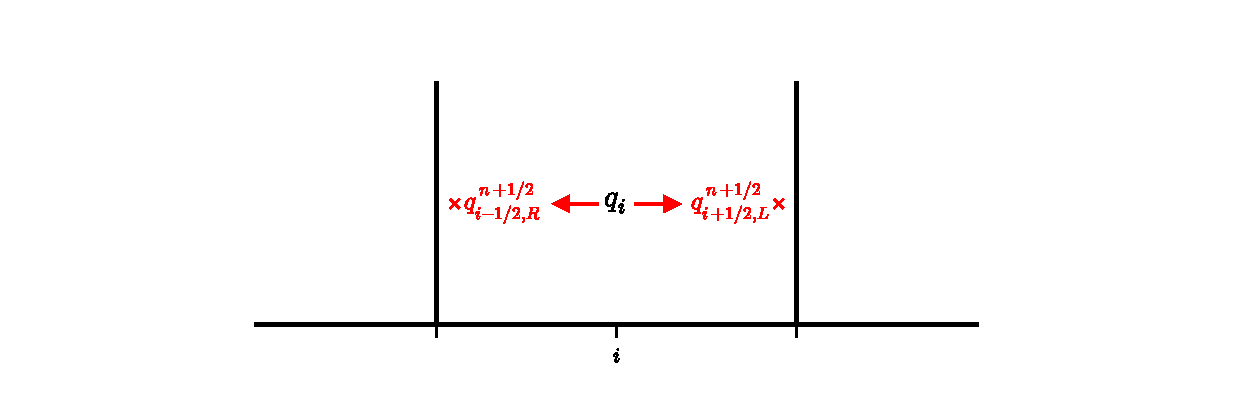
\includegraphics[width=3.5in]{states}
\caption[The two interface states derived from a cell-center quantity.]{\label{fig:states} The two interface states that are constructed
using $q_i$ as the starting point.}
\end{figure}

\subsection{Piecewise parabolic}

The piecewise parabolic method uses a parabolic reconstruction in each
cell.  This is more accurate than the linear reconstruction.
Figure~\ref{fig:ppm} shows the reconstructed parabolic profiles within
a few cells.  Since the original PPM
paper~\cite{colellawoodward:1984}, there have been many discussions of
the method, with many variations.  Here we focus on the presentation
by Miller \& Colella~\cite{millercolella:2002}, since that is the most
straightforward.  Note: even though a parabolic profile could be
third-order accurate, the temporal discretization and prediction in
this method is still only second-order.
%
\begin{figure}[t]
\centering
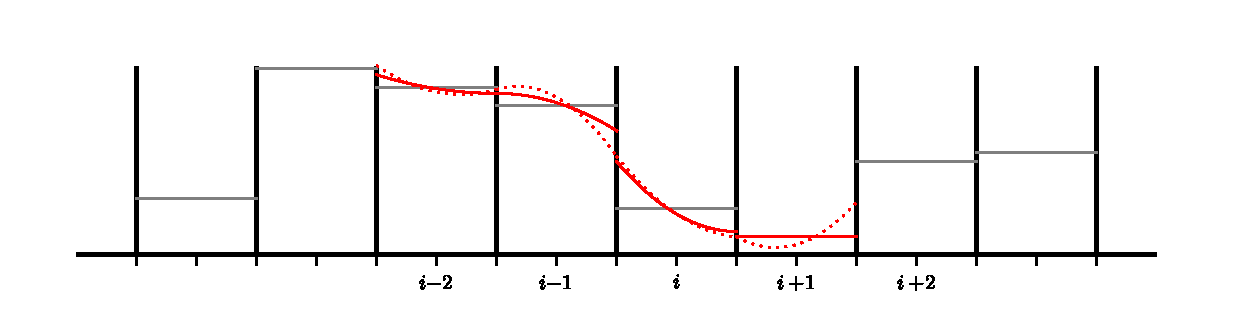
\includegraphics[width=\linewidth]{piecewise-parabolic}
\caption[Piecewise parabolic reconstruction of the cell
  averages.]{\label{fig:ppm} Piecewise parabolic reconstruction of the
  cell averages.  The dotted line shows the unlimited parabolas---note
  how they touch at each interface, since the interface values come
  from the same interpolant initially.  The solid line shows the
  limited parabolas.}
\end{figure}


Miller \& Colella give an excellent description of how to take the
results for piecewise linear reconstruction and generalize it to the case of
PPM~\cite{colellawoodward:1984} (see Eqs.\ 88-90).  Starting with
Eq.~\ref{eq:lin_decomp}, we can write this (after the characteristic
projection) as
\begin{equation}
q_{i+1/2,L}^{n+1/2} = \tilde{q}_+ -
   \sum_{\nu;\lambda^{(\nu)}\ge 0} l_i^{(\nu)} \cdot \left \{
        \tilde{q}_+ - \left [ q_i^n +
            \frac{1}{2} \left ( 1 - \frac{\Delta t}{\Delta x} \lambda_i^{(\nu)} \right ) \overline{\Delta q}_i \right ]
       \right \} r_i^{(\nu)}
\end{equation}
Miller \& Colella rewrite the portion inside the $[\ldots]$
recognizing that (similar to M\&C Eq.\ 88, but for the $i+1/2,L$ interface):
\begin{equation}
  q_i^n + \frac{1}{2} \left (1 - \frac{\Delta t}{\Delta x} \lambda_i^{(\nu)} \right ) \overline{\Delta q}_i 
  \approx \frac{1}{\lambda \Delta t} \int_{x_{i+1/2} - \lambda \Delta t}^{x_{i+1/2}}
           q(x) dx
\end{equation}
where $q(x)$ is the reconstructed functional form of $q$ in the zone.

\begin{exercise}[The average state reacting the interface]
{Show that this is exactly true for a linear reconstruction of $q(x)$, i.e.,
$q(x) = q_i + (\partial q/\partial x) (x - x_i)$.}
\end{exercise}

\noindent The integral on the right represents the average of $q$ that
can reach the right interface of the cell $i$ over timestep $\Delta
t$, moving at the wavespeed $\lambda$.  This suggests that we can
replace the linear reconstruction of $q$ with a parabolic one, and
keep our expressions for the interface states.

\begin{figure}
\centering
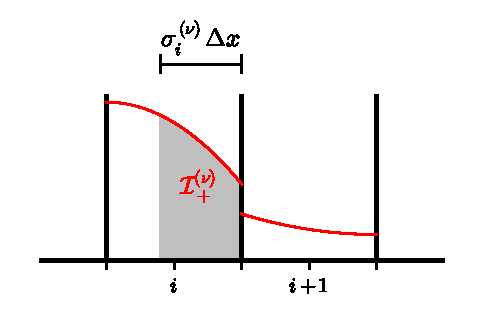
\includegraphics[width=3.5in]{ppm-trace}
\caption[Integration under the parabola profile for to an
  interface.]{\label{fig:ppm_trace} Integration under the parabolic
  profile.  For each of the waves, $\sigma^\enu$ is the fraction of
  the cell that they cross in a timestep, and $\sigma^\enu \Delta x =
  \lambda^\enu \Delta t$ is the distance they can travel.  Here we are
  integrating under the parabola to the right interface of cell $i$ to
  define $\mathcal{I}_+^\enu$ (this is indicated by the shaded
  region).  The $\mathcal{I}_+^\enu$ carried by this wave will be
  added to those carried by the other waves to form the left state at
  interface $i+1/2$.}
\end{figure}

In particular, we define 
\begin{equation}
\mathcal{I}_+^{(\nu)}(q_i) = \frac{1}{\sigma^{(\nu)} \Delta x} \int _{x_{i+1/2} - \sigma^{(\nu)} \Delta x}^{x_{i+1/2}} q(x) dx
\end{equation} 
with $\sigma^{(\nu)} = |\lambda^{(\nu)}|\Delta t / \Delta x$ (see Almgren et
al. Eq. 31)  (see Figure~\ref{fig:ppm_trace}).  Then
\begin{equation}
q_{i+1/2,L}^{n+1/2} = \tilde{q}_+ -
   \sum_{\nu;\lambda^{(\nu)}\ge 0} l_i^{(\nu)} \cdot \left (
        \tilde{q}_+ - \mathcal{I}_+^{(\nu)}(q_i)
       \right ) r_i^{(\nu)}  \label{eq:ppmtrace}
\end{equation}
Miller \& Colella choose the reference state as
\begin{equation}
\tilde{q}_+ = \left \{ \begin{array}{cc} 
       \mathcal{I}_+^{(+)}(q_i) & \mathrm{if~} u + c > 0 \\
       q_i                    & \mathrm{otherwise}
\end{array}
\right .
\end{equation}
where the superscript $(+)$ on $\mathcal{I}$ indicates that the
fastest eigenvalue ($\lambda^\evp = u + c$) is used.  This is similar in
spirit to Eq.~\ref{eq:qref}.  Note: in the original PPM paper, if the
wave is not approaching the interface, instead of using the
cell-average, $q_i$, they use the limit of the quadratic interpolant.
In contrast to the above, the Castro paper~\cite{almgren:2010} just
uses $q_i$ for the reference state regardless of whether the wave is
moving toward or away from the interface.  Note that if the system
were linear, then the choice of reference state would not matter.

To finish the reconstruction, we need to know the parabolic form
of $q(x)$.  Here, we do the reconstruction from the original PPM
paper:
\begin{equation}
q(x) = q_{-} + \xi(x) \left ( \Delta q + q_6 (1 - \xi(x) ) \right )
\end{equation}
with $\Delta q = q_+ - q_-$, and $q_-$, $q_+$ the values of the polynomial
on the left and right edges, respectively, of the current cell, and 
\begin{equation}
q_6 \equiv 6 \left [ q_i - \frac{1}{2} (q_- + q_+) \right ]
\end{equation}
and
\begin{equation}
\xi(x) = \frac{x - x_{i-1/2}}{\Delta x}
\end{equation}

To complete the description, we need to determine the parameters of
the parabola.  The values of $q_-$ and $q_+$ are computed and limited
as described in the original PPM paper.  With this definition, we can
do the integral $\mathcal{I}_+$:
\begin{equation}
\mathcal{I}_+^{(\nu)}(q_i) = q_{+,i} - \frac{\sigma_i^{(\nu)}}{2} 
   \left [ \Delta q_i - q_{6,i} \left ( 1 - \frac{2}{3} \sigma_i^{(\nu)} \right ) \right ]
\end{equation}
Figure~\ref{fig:ppm_trace} illustrates the process of integrating under
the parabolic profile.


\begin{exercise}[Conservative interpolation]
{Show that $q(x)$ is a conservative interpolant.  That is
\begin{equation}
\frac{1}{\Delta x} \int_{x_{i-1/2}}^{x_{i+1/2}} q(x) dx = q_i
\end{equation}
You can also see that the average over the left half of the zone is
$q_i -\frac{1}{4}\Delta q$ and the average over the right half of the
zone is $q_i + \frac{1}{4}\Delta q$.  This means that there are equal
areas between the integral and zone average on the left and right
sides of the zone.  This can be seen by looking at
Figure~\ref{fig:ppm}.  }
\end{exercise}

\begin{quote}
\noindent\makebox[\linewidth]{\rule{0.9\textwidth}{1pt}} 
{\em Aside}: 
Note that this characteristic projection of $\tilde{q}_+ -
\mathcal{I}_+^{(\nu)}$ is discussed in the original PPM paper in the
paragraph following Eq. 3.5.  They do not keep things in this form
however, and instead explicitly multiply out the $l\cdot [\ldots] r$
terms to arrive at Eq. 3.6.  For example, starting with
Eq.~\ref{eq:ppmtrace}, 
we can write the left velocity state as (leaving off the $i$
subscripts on the vectors):
\begin{equation}
u_{i+1/2,L}^{n+1/2} = 
  \tilde{u}_+ - \sum_\nu l^{(\nu)} \cdot 
      ( \tilde{q}_+ -  \mathcal{I}_+^{(\nu)}(q) ) 
    \underbrace{r^{(\nu)}}_{\begin{smallmatrix}\mathrm{only~the}\\ u~\mathrm{`slot'} \end{smallmatrix}}
\end{equation}
(where, as above, the $\sim$ indicates the reference state).
Here the $r$ eigenvector on the end is representative---we only pick
the row corresponding to $u$ in the $q$ vector (in our case, the
second row).  

Putting in the eigenvectors and writing out the sum, we have:
\begin{align}
 u_{i+1/2,L}^{n+1/2} =
     \tilde{u}_+ &- 
       \left ( \begin{array}{ccc} 
                  0 & -\frac{\rho}{2c} & \frac{1}{2c^2} \end{array} 
       \right ) 
    \left ( \begin{array}{c} 
           \tilde{\rho}_+ - \mathcal{I}_+^\evm(\rho) \\
           \tilde{u}_+ - \mathcal{I}_+^\evm(u) \\
           \tilde{p}_+ - \mathcal{I}_+^\evm(p) 
            \end{array} \right )
    {\color{mygray} \left ( \begin{array}{c} 
           1  \\
           {\color{black} -c/\rho} \\
           c^2
    \end{array} \right ) } \nonumber \\
%
     &-\left ( \begin{array}{ccc} 
                  1 & 0 & -\frac{1}{c^2} \end{array} 
       \right ) 
    \left ( \begin{array}{c} 
           \tilde{\rho}_+ - \mathcal{I}_+^\evz(\rho) \\
           \tilde{u}_+ - \mathcal{I}_+^\evz(u) \\
           \tilde{p}_+ - \mathcal{I}_+^\evz(p) 
            \end{array} \right )
    {\color{mygray} \left ( \begin{array}{c} 
           1  \\
           {\color{black} 0} \\
           0
    \end{array} \right ) } \nonumber \\
%
    &-\left ( \begin{array}{ccc} 
                  0 & \frac{\rho}{2c} & \frac{1}{2c^2} \end{array} 
       \right ) 
    \left ( \begin{array}{c} 
           \tilde{\rho}_+ - \mathcal{I}_+^\evp(\rho) \\
           \tilde{u}_+ - \mathcal{I}_+^\evp(u) \\
           \tilde{p}_+ - \mathcal{I}_+^\evp(p) 
            \end{array} \right )
    {\color{mygray} \left ( \begin{array}{c} 
           1  \\
           {\color{black} c/\rho} \\
           c^2
    \end{array} \right ) } 
%
\end{align}
Here again we show the entire right eigenvector for illustration, but
only the element that comes into play is drawn in black.  This shows
that the second term is $0$---the contact wave does not carry a jump
in velocity.  Multiplying out $l^{(\nu)} \cdot (\tilde{q}_+ -
\mathcal{I}_+^{(\nu)})$ we have:
\begin{align}
u_{i+1/2,L}^{n+1/2} =
   \tilde{u}_+ 
  &- \frac{1}{2} \left [
      (\tilde{u}_+ - \mathcal{I}_+^\evm(u) ) - 
       \frac{\tilde{p}_+ - \mathcal{I}_+^\evm(p)}{C} \right ] \nonumber \\
  &- \frac{1}{2} \left [
      (\tilde{u}_+ - \mathcal{I}_+^\evp(u) ) +
       \frac{\tilde{p}_+ - \mathcal{I}_+^\evp(p)}{C} \right ]
\label{eq:ufull}
\end{align}
where $C$ is the Lagrangian sound speed ($C = \sqrt{\gamma p \rho}$).
Defining 
\begin{align}
\beta^{+} &= - \frac{1}{2C}
  \left [
      (\tilde{u}_+ - \mathcal{I}_+^\evp(u) ) +
       \frac{\tilde{p}_+ - \mathcal{I}_+^\evp(p)}{C} \right ] \\
%
\beta^{-} &= + \frac{1}{2C}
  \left [
      (\tilde{u}_+ - \mathcal{I}_+^\evm(u) ) -
       \frac{\tilde{p}_+ - \mathcal{I}_+^\evm(p)}{C} \right ]
\end{align}
we can write our left state as:
\begin{equation}
u_{i+1/2,L}^{n+1/2} =
   \tilde{u}_+ + C ( \beta^+ - \beta^-)
\end{equation}
This is Eqs.~3.6 and 3.7 in the PPM paper.  Note that in their
construction appears to use the reference state in defining the
Lagrangian sound speed (in their $\beta$ expressions is written as
$\tilde{C}$).  This may follow from the comment before Eq.~3.6,
``modified slightly for the present application''.  Similarly,
the expressions for $\rho_L$ and $p_L$ can be written out. \\
\noindent\makebox[\linewidth]{\rule{0.9\textwidth}{1pt}} 
\end{quote}

Similar expressions can be derived for the right state at the left interface
of the zone ($q_{i-1/2,R}^{n+1/2}$).  Here, the integral under the parabolic
reconstruction is done over the region of each wave that can reach the left 
interface over our timestep:
\begin{equation}
\mathcal{I}_-^{(\nu)}(q) = \frac{1}{\sigma^{(\nu)} \Delta x}
  \int_{x_{i-1/2}}^{x_{i-1/2} + \sigma^{(\nu)} \Delta x} q(x) dx
\end{equation}
The right state at $i-1/2$ using zone $i$ data is:
\begin{equation}
q_{i-1/2,R}^{n+1/2} = \tilde{q}_- - \sum_{\nu; \lambda_\nu \le 0}
   l_i^{(\nu)} \cdot \left ( \tilde{q}_- - \mathcal{I}_-^{(\nu)}(q_i) \right ) r_i^{(\nu)}
\end{equation}
where the reference state is now:
\begin{equation}
\tilde{q}_- = \left \{ \begin{array}{cc}
   \mathcal{I}_-^{(-)}(q_i) & \mathrm{if~} u - c < 0 \\
    q_i                   & \mathrm{otherwise}
\end{array} \right .
\end{equation}
where the $(-)$ superscript on $\mathcal{I}$ indicates that the most
negative eigenvalue $(\lambda^- = u - c)$ is used.  The integral
$\mathcal{I}_-^{(\nu)}(q)$ can be computed analytically by
substituting in the parabolic interpolant, giving:
\begin{equation}
\mathcal{I}_-^{(\nu)}(q_i) = q_{-,i} + \frac{\sigma_i^{(\nu)}}{2}
   \left [ \Delta q_i + q_{6,i} \left ( 1 - \frac{2}{3} \sigma_i^{(\nu)} \right ) \right ]
\end{equation}
This is equivalent to Eq.~31b in the Castro paper.

%-----------------------------------------------------------------------------
\section{The Riemann problem}

Once the interface states are created, the Riemann solver is called.  This 
returns the solution at the interface:
\begin{equation}
q_{i+1/2}^{n+1/2} = \mathcal{R}(q_{i+1/2,L}^{n+1/2}, q_{i+1/2,R}^{n+1/2})
\end{equation}

Solving the Riemann problem for the Euler equations can be a complex
operation, but the general ideas are straightforward.  Here we review
the basic outline of operations, and refer to Toro~\cite{toro:1997} for
full details on a variety of methods for solving the Riemann problem.

The Riemann problem consists of a left and right state separated by an
interface.  For the Euler equations, there are three eigenvalues, which
are the speeds at which information propagates.  Each of these
correspond to a wave that will move out from the interface with time,
and each wave will carry with it a jump in the characteristic variables.  The
figure below shows the three waves moving out from the interface,
separating space into 4 regions, marked: $L$, $L^*$, $R^*$, and $R$.
\begin{figure}[h]
\centering
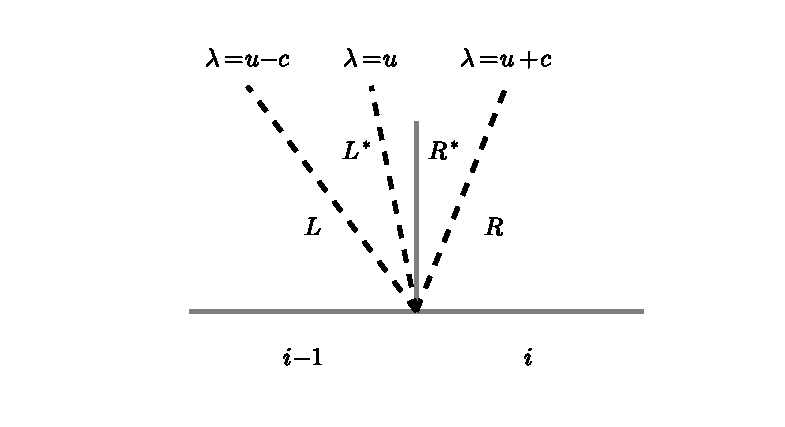
\includegraphics[width=4.5in]{riemann-waves}
\caption[The Riemann problem wave struction for the Euler
  equations.]{The wave structure and 4 distinct regions for the
  Riemann problem.  Time can be thought of as the vertical axis here,
  so we see the waves moving outward from the interface.}
\end{figure} 
We typically work in terms of primitive variables.  The states in the
$L$ and $R$ regions are simply the left and right input states---the
waves have not had time to reach here, so they are unmodified.

The left and right states are connected to the state in the star
region by a Hugoniot curve---this is a curve in the $u$-$p$
plane that shows all of the possible states one can reach from 
the current state through either a shock or rarefaction.  There
are two such curves, one corresponding to the left and one to the right
state, and the solution to the Riemann problem is the point in
the $u$-$p$ plane where these two curves intersect.  Figure~\ref{fig:euler:riemann-curve}
shows the Hugoniot curves for the Sod problem.

\begin{figure}[t]
\centering
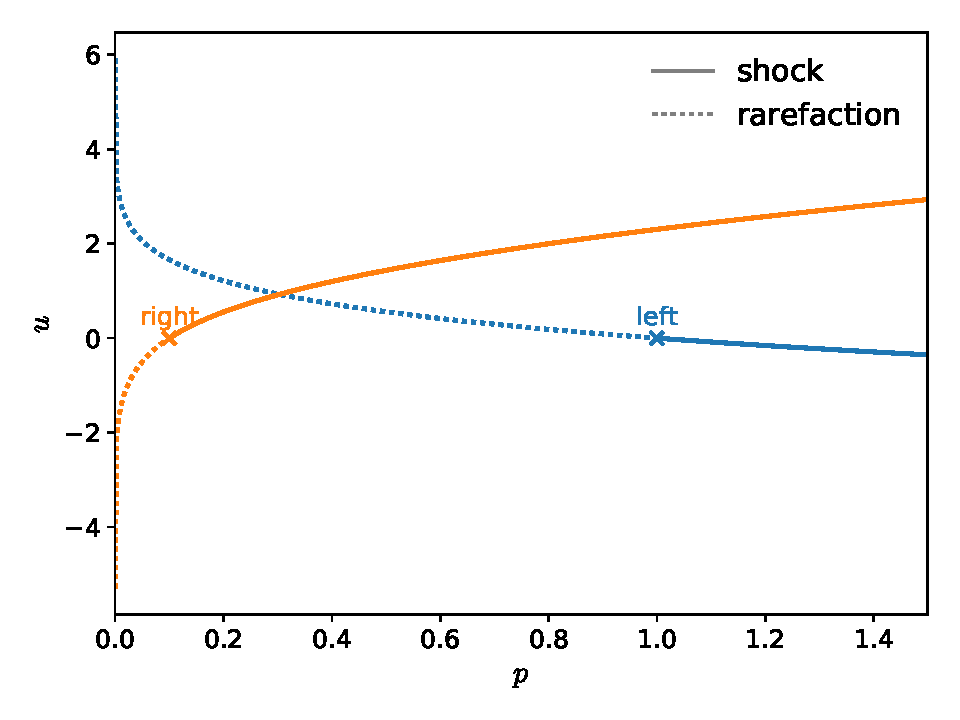
\includegraphics[width=0.8\linewidth]{riemann-phase}
\caption[The Hugoniot curves corresponding
to the Sod problem.]{\label{fig:euler:riemann-curve} The Hugoniot curves corresponding
to the Sod problem.  The shock and rarefaction curves are shown.  The
solution to the Riemann problem is the point where the curves intersect.\\
\hydroexdoit{\href{https://github.com/zingale/hydro_examples/blob/master/compressible/riemann-phase.py}{riemann-phase.py}}}
\end{figure}

We are interested in the state at the interface.  To
determine this, we need to determine which region we are in.  That
requires an estimation of the wave speeds.  Since these are nonlinear
waves, we cannot in general just use the eigenvalues (although some
approximate solvers do).  Different Riemann solvers will have
different approximations for finding the speeds of the left, center,
and right wave.  Note the figure shows only one possible configuration
for the waves---they can all be on one side of the interface (for
all supersonic waves), or the contact (the middle wave) can be on either
side.

Once the wave speeds are known, we look at the sign of the speeds to
determine which of the 4 regions is on the interface.  In the `star'
region, only $\rho$ jumps across the middle (contact) wave, the
pressure and velocity are constant across that wave (see $r^\evz$).
We determine the state in the star region ($\rho_l^*, \rho_r^*, u^*,
p^*$) by using the jump conditions for the Euler equations.  In
general, these differ depending on whether the waves are shocks or
rarefactions.  In practice, approximate Riemann solvers often assume
one or the other (for example, the two-shock Riemann solver used
in~\cite{colellaglaz:1985}).  With the wave speeds and the states
known in each region, we can evaluate the state on the interface,
$q_{i+1/2}^{n+1/2}$.

Recall that a rarefaction involves diverging flow---it spreads out
with time.  Special consideration needs to be taken if the rarefaction
wave spans the interface (a {\em transonic rarefaction}).  In this
case, most Riemann solvers interpolate between the left or right state
and the appropriate star state.

Then the fluxes are computed from this state as:
\begin{equation}
\renewcommand{\arraystretch}{1.5}
F_{i+1/2}^{n+1/2} = \left ( \begin{array}{c}
                             \rho_{i+1/2}^{n+1/2} u_{i+1/2}^{n+1/2} \\
                             \rho_{i+1/2}^{n+1/2} (u_{i+1/2}^{n+1/2})^2 + p_{i+1/2}^{n+1/2} \\
                             u_{i+1/2}^{n+1/2} p_{i+1/2}^{n+1/2} / (\gamma - 1)  +
                             \frac{1}{2} \rho_{i+1/2}^{n+1/2} (u_{i+1/2}^{n+1/2})^3 +
                             u_{i+1/2}^{n+1/2} p_{i+1/2}^{n+1/2}
                            \end{array} \right )
\renewcommand{\arraystretch}{1.0}
\end{equation}

Note that instead of returning an approximate state at the interface,
some Riemann solvers (e.g.\ the HLL(C) solvers) instead approximate the
fluxes directly.

%-----------------------------------------------------------------------------
\section{Conservative update}

Once we have the fluxes, the conservative update is done as
\begin{equation}
U^{n+1}_i = U^n_i + \frac{\Delta t}{\Delta x} \left ( F_{i-1/2}^{n+1/2} - F_{i+1/2}^{n+1/2} \right )
\end{equation}
The timestep, $\Delta t$ is determined by the time it takes for the fastest
wave to cross a single zone:
\begin{equation}
\Delta t < \max_i \frac{\Delta x}{|u_i| + c}
\end{equation}
              


%-----------------------------------------------------------------------------
\section{Multidimensional problems}

The multidimensional case is very similar to the multidimensional
advection problem.  Our system of equations is now:
\begin{equation}
U_t + [F^{(x)}(U)]_x + [F^{(y)}(U)]_y = 0
\end{equation}
with
\begin{equation}
U = \left ( \begin{array}{c} \rho \\ \rho u \\ \rho v \\ \rho E \end{array} \right )
%
\qquad
%
F^{(x)}(U) = \left ( \begin{array}{c} \rho u \\ \rho uu + p \\ \rho v u \\ \rho u E + up \end{array} \right )
%
\qquad
F^{(y)}(U) = \left ( \begin{array}{c} \rho v \\ \rho vu     \\ \rho v v + p \\ \rho v E + vp \end{array} \right )
\end{equation}

We note that there is no transformation that can convert the multidimensional
system into characteristic variables, since we cannot simultaneously 
diagonalize the Jacobians corresponding to $F^{(x)}$ and $F^{(y)}$.  Related
to this is that when limiting, we limit one-dimensional slopes instead of
doing a full multidimensional reconstruction and limiting (see \cite{BDS} 
for a multidimensional limiting procedure for linear advection.  For
the Euler equations, since we cannot write the multidimensional system
in a characteristic form, we cannot use this type of method).

For a directionally-unsplit discretization, we predict the
cell-centered quantities to the edges by Taylor expanding the
conservative state, $U$, in space and time.  Now, when replacing the
time derivative ($\partial U/\partial t$) with the divergence of the
fluxes, we gain a transverse flux derivative term.  For example,
predicting to the upper $x$ edge of zone $i,j$, we have:
\begin{align}
U_{i+1/2,j,L}^{n+1/2} &= U_{i,j}^n + \frac{\Delta x}{2} \frac{\partial U}{\partial x} 
                            + \frac{\Delta t}{2} \frac{\partial U}{\partial t} + \ldots \\
&= U_{i,j}^n + \frac{\Delta x}{2} \frac{\partial U}{\partial x} 
                            - \frac{\Delta t}{2} \frac{\partial F^{(x)}}{\partial x} 
                            - \frac{\Delta t}{2} \frac{\partial F^{(y)}}{\partial y} \\
&= U_{i,j}^n + \frac{1}{2} \left [ 1 - \frac{\Delta t}{\Delta x} A^{(x)}(U) \right ] \Delta U 
                            - \frac{\Delta t}{2} \frac{\partial F^{(y)}}{\partial y} \label{eq:Utaylorstate}
\end{align}
where $A^{(x)}(U) \equiv \partial F^{(x)} / \partial U$.  We decompose
this into a {\em normal state} and a {\em transverse flux difference}.
Adopting the notation from Colella (1990), we use $\hat{U}$ to denote
the normal state:
\begin{align}
\hat{U}_{i+1/2,j,L}^{n+1/2} &\equiv U_{i,j}^n 
      + \frac{1}{2} \left [ 1 - \frac{\Delta t}{\Delta x} A^{(x)}(U) \right ] \Delta U \\
U_{i+1/2,j,L}^{n+1/2} &= \hat{U}_{i+1/2,j,L}^{n+1/2}
                            - \frac{\Delta t}{2} \frac{\partial F^{(y)}}{\partial y}  \label{eq:fullleftstate}
\end{align}

The primitive variable form for this system is
\begin{equation}
q_t + A^{(x)}(q) q_x + A^{(y)}(q) q_y = 0
\end{equation}
where
\begin{equation}
q = \left ( \begin{array}{c} \rho \\ u \\ v \\ p \end{array} \right )
%
\qquad
A^{(x)}(q) = \left ( \begin{array}{cccc} u  & \rho     & 0 &  0 \\
                                         0  &  u       & 0 &  1/\rho \\
                                         0  &  0       & u &  0 \\
                                         0  & \gamma p & 0 &  u \end{array} \right )
\qquad
A^{(y)}(q) = \left ( \begin{array}{cccc} v  & 0 & \rho &  0 \\
                                         0  & v & 0    &  0 \\
                                         0  & 0 & v    &  1/\rho \\
                                         0  & 0 & \gamma p & v \end{array} \right )
\end{equation}
There are now 4 eigenvalues.  For $A^{(x)}(q)$, they are $u-c$, $u$,
$u$, $u+c$.  If we just look at the system for the $x$ evolution, we
see that the transverse velocity (in this case, $v$) just advects with
velocity $u$, corresponding to the additional eigenvalue.
\begin{exercise}[Eigenvectors for the 2-d Euler equations]
{
Derive the form of $A^{(x)}(q)$ and $A^{(y)}(q)$ and find their left and right eigenvectors.}
\end{exercise}

We note here that $\hat{U}_{i+1/2,j,L}^{n+1/2}$ is essentially
one-dimensional, since only the $x$-fluxes are involved (through
$A^{(x)}(U)$).  This means that we can compute this term using the
one-dimensional techniques developed in \S~\ref{sec:onedrecon}.  In
particular, Colella (1990) suggest that we switch to primitive variables
and compute this as:
\begin{equation}
\hat{U}_{i+1/2,j,L}^{n+1/2} = U(\hat{q}_{i+1/2,j,L}^{n+1/2})
\end{equation}
Similarly, we consider the system projected along the $y$-direction to
define the normal states on the $y$-edges, again using the one-dimensional
reconstruction on the primitive variables from \S~\ref{sec:onedrecon}:
\begin{equation}
\hat{U}_{i,j+1/2,L}^{n+1/2} = U(\hat{q}_{i,j+1/2,L}^{n+1/2})
\end{equation}

To compute the full interface state (Eq.~\ref{eq:fullleftstate}), we 
need to include the transverse term.
Colella (1990) gives two different procedures for evaluating the
transverse fluxes.  The first is to simply use the cell-centered
$U_{i,j}$ (Colella 1990,
Eq. 2.13); the second is to use the reconstructed normal states (the
$\hat{U}$'s) (Eq. 2.15).  In both cases, we need to solve a {\em
  transverse Riemann problem} to find the true state on the transverse
interface.  This latter approach is what we prefer.  In particular, 
for computing the full $x$-interface left state, $U_{i+1/2,j,L}^{n+1/2}$, we need the 
transverse ($y$) states, which we define as
\begin{align}
U^T_{i,j+1/2} &= \mathcal{R}(\hat{U}^{n+1/2}_{i,j+1/2,L}, 
                            \hat{U}^{n+1/2}_{i,j+1/2,R}) \\
U^T_{i,j-1/2} &= \mathcal{R}(\hat{U}^{n+1/2}_{i,j-1/2,L}, 
                            \hat{U}^{n+1/2}_{i,j-1/2,R})
\end{align}

Taken together, the full interface state is now:
\begin{equation}
U_{i+1/2,j,L}^{n+1/2} = U(\hat{q}_{i+1/2,j,L}^{n+1/2}) 
   - \frac{\Delta t}{2} \frac{F^{(y)}(U^T_{i,j+1/2}) - F^{(y)}(U^T_{i,j-1/2})}{\Delta y}
\end{equation}

The right state at the $i+1/2$ interface can be similarly computed (starting with the
data in zone $i+1,j$ and expanding to the left) as:
\begin{equation}
U_{i+1/2,j,R}^{n+1/2} = U(\hat{q}_{i+1/2,j,R}^{n+1/2}) 
   - \frac{\Delta t}{2} \frac{F^{(y)}(U^T_{i+1,j+1/2}) - F^{(y)}(U^T_{i+1,j-1/2})}{\Delta y}
\end{equation}
Note the indices on the transverse states---they are now to the right of the interface (since
we are dealing with the right state).

We then find the $x$-interface state by solving the Riemann problem
normal to our interface:
\begin{equation}
U_{i+1/2,j}^{n+1/2} = \mathcal{R}(U_{i+1/2,j,L}^{n+1/2}, U_{i+1/2,j,R}^{n+1/2})
\end{equation}
Therefore, construction of the interface states now requires two
Riemann solves: a transverse and normal one.  The fluxes are then evaluated as:
\begin{equation}
F^{(x),n+1/2}_{i+1/2,j} = F^{(x)}(U_{i+1/2,j}^{n+1/2})
\end{equation}
Note, for multi-dimensional problems, in the Riemann solver, the transverse
velocities are simply selected based on the speed of the contact, giving
either the left or right state.
 
The final conservative update is done as:
\begin{equation}
U^{n+1}_{i,j} = U^n_{i,j} 
   + \frac{\Delta t}{\Delta x} \left ( F^{(x),n+1/2}_{i-1/2,j} - F^{(x),n+1/2}_{i+1/2,j} \right )
   + \frac{\Delta t}{\Delta y} \left ( F^{(y),n+1/2}_{i,j-1/2} - F^{(y),n+1/2}_{i,j+1/2} \right )
\end{equation}


%-----------------------------------------------------------------------------
\section{Boundary conditions}

Boundary conditions are implemented through ghost cells.  The following
are the most commonly used boundary conditions.  For the expressions
below, we use the subscript $\mathrm{lo}$ to denote the spatial index
of the first valid zone in the domain (just inside the left boundary).

\begin{itemize}

\item {\em Outflow}: the idea here is that the flow should gracefully
  leave the domain.  The simplest form is to simply give all variables
  a zero-gradient:
  \begin{equation}
  \left ( \begin{array}{c} \rho_{\mathrm{lo-1},j} \\ 
                           (\rho u)_{\mathrm{lo-1},j} \\ 
                           (\rho v)_{\mathrm{lo-1},j} \\
                           (\rho E)_{\mathrm{lo-1},j} \end{array} \right ) =
  \left ( \begin{array}{c} \rho_{\mathrm{lo},j} \\ 
                           (\rho u)_{\mathrm{lo},j} \\ 
                           (\rho v)_{\mathrm{lo},j} \\
                           (\rho E)_{\mathrm{lo},j} \end{array} \right )
  \end{equation}

  Note that these boundaries are not perfect.  At the boundary, one
  (or more) of the waves from the Riemann problem can still enter
  the domain.  Only for supersonic flow, do all waves point outward.


\item {\em Reflect}: this is appropriate at a solid wall or symmetry
  plane.  All variables are reflected across the boundary, with the
  normal velocity given the opposite sign.  At the $x$-boundary, the
  first ghost cell is:
  \begin{equation}
  \left ( \begin{array}{c} \rho_{\mathrm{lo-1},j} \\ 
                           (\rho u)_{\mathrm{lo-1},j} \\ 
                           (\rho v)_{\mathrm{lo-1},j} \\
                           (\rho E)_{\mathrm{lo-1},j} \end{array} \right ) =
  \left ( \begin{array}{c} \rho_{\mathrm{lo},j} \\ 
                           -(\rho u)_{\mathrm{lo},j} \\ 
                           (\rho v)_{\mathrm{lo},j} \\
                           (\rho E)_{\mathrm{lo},j} \end{array} \right )
  \end{equation}
  The next is:
  \begin{equation}
  \left ( \begin{array}{c} \rho_{\mathrm{lo-2},j} \\ 
                           (\rho u)_{\mathrm{lo-2},j} \\ 
                           (\rho v)_{\mathrm{lo-2},j} \\
                           (\rho E)_{\mathrm{lo-2},j} \end{array} \right ) =
  \left ( \begin{array}{c} \rho_{\mathrm{lo+1},j} \\ 
                           -(\rho u)_{\mathrm{lo+1},j} \\ 
                           (\rho v)_{\mathrm{lo+1},j} \\
                           (\rho E)_{\mathrm{lo+1},j} \end{array} \right )
  \end{equation}
  and so on $\ldots$


  \item {\em Inflow}: inflow boundary conditions specify the state
    directly on the boundary.  Technically, this state is on the
    boundary itself, not the cell-center.  This can be accounted for
    by modifying the stencils used in the reconstruction near inflow
    boundaries.

  \item {\em Hydrostatic}: a hydrostatic boundary can be used at the
    base of an atmosphere to provide the pressure support necessary to
    hold up the atmosphere against gravity while still letting
    acoustic waves pass through.  An example of this is described
    in \cite{hse}.

\end{itemize}


%-----------------------------------------------------------------------------
\section{Going further}

\label{sec:euler:further}

\begin{itemize}

\item {\em Flattening}: shocks are self-steepening (this is how we
  detect them in the Riemann solver---we look for converging characteristics).
  This can cause trouble with the methods here, because the shocks may become
  too steep.  

  Flattening is a procedure to add additional dissipation at shocks,
  to ensure that they are smeared out over $\sim 2$ zones.  The
  flattening procedure is a multi-dimensional operation that looks at
  the pressure and velocity profiles and returns a coefficient, $\chi
  \in [0,1]$ that multiplies the limited slopes.  The convention most
  sources use is that $\chi = 1$ means no flattening (the slopes are
  unaltered), while $\chi = 0$ means complete flattening---the slopes
  are zeroed, dropping us to a first-order method.
  See for example in Saltzman~\cite{saltzman:1994}.  Once the flattening
  coefficient is determined, the interface state is blended with the
  cell-centered value via:
  \begin{equation}
  q_{i+1/2,\{L,R\}}^{n+1/2} \leftarrow (1 - \chi) q_i + \chi q_{i+1/2,\{L,R\}}^{n+1/2}
  \end{equation}

  Note that the flattening algorithm increases the stencil size of
  piecewise-linear and piecewise-parabolic reconstruction to 4 ghost cells
  on each side.  This is because the flattening procedure itself looks
  at the pressure 2 zones away, and we need to construct the flattening
  coefficient in both the first ghost cell (since we need the interface
  values there) and the second ghost cell (since the flattening procedure
  looks at the coefficients in its immediate upwinded neighbor).

\item {\em Artificial viscosity}: Colella and Woodward argue discuss
  that behind slow-moving shocks these methods can have oscillations.
  The fix they propose is to use some artificial viscosity---this is
  additional dissipation that kicks in at shocks.  (They argue that
  flattening alone is not enough).  

  We use a multidimensional analog of their artificial viscosity
  (\cite{colellawoodward:1984}, Eq.\ 4.5) which modifies the fluxes.
  By design, it only kicks in for converging flows, such that you
  would find around a shock.

\item {\em Contact steepening}: in contrast to shocks, contact waves
  do not steepen (they are associated with the middle characteristic
  wave, and the velocity does not change across that, meaning there
  cannot be any convergence).  The original PPM
  paper advocates a contact steepening method to artificially steepen
  contact waves.  While it shows good results in 1-d, it can be
  problematic in multi-dimensions.  

  Overall, the community seems split over whether this term should be
  used.  Many people advocate that if you reach a situation where you
  think contact steepening may be necessary, it is more likely that
  the issue is that you do not have enough resolution.

\item {\em Species}: for multifluid flows, the Euler equations are
augments with continuity equations for each of the (chemical or nuclear)
species:
\begin{equation}
\frac{\partial (\rho X_k)}{\partial t} + \frac{\partial (\rho X_k u)}{\partial x} = 0
\end{equation}
here, $X_k$ are the mass fractions and obey $\sum_k X_k = 1$.  Using the
continuity equation, we can write this as an advection equation:
\begin{equation}
\frac{\partial X_k}{\partial t} + u \frac{\partial X_k}{\partial x} = 0
\end{equation}
When we now consider our primitive variables: $q = (\rho, u, p, X_k)$,
we find
\begin{equation}
A(q) = \left ( \begin{array}{cccc} u  & \rho     & 0      &  0\\
                                  0  &  u       & 1/\rho &  0\\
                                  0  & \gamma p & u      &  0\\
                                  0  & 0        & 0      & u \end{array} \right )
\end{equation}
There are now 4 eigenvalues, with the new one also being simply $u$.
This says that the species simply advect with the flow.  The right
eigenvectors are now:
\begin{equation}
r^{(1)} = \left ( \begin{array}{c} 1 \\ -c/\rho \\ c^2 \\ 0\end{array} \right )
%
\qquad
r^{(2)} = \left ( \begin{array}{c} 1 \\ 0 \\ 0  \\ 0\end{array} \right )
%
\qquad
r^{(3)} = \left ( \begin{array}{c} 0 \\ 0  \\ 0 \\ 1 \end{array} \right )
%
\qquad
r^{(4)} = \left ( \begin{array}{c} 1 \\ c/\rho \\ c^2 \\ 0 \end{array} \right )
\end{equation}
corresponding to $\lambda^{(1)} = u -c$, $\lambda^{(2)} = u$,
$\lambda^{(3)} = u$, and $\lambda^{(4)} = u + c$.  We see that for the
species, the only non-zero element is for one of the $u$ eigenvectors.
This means that $X_k$ only jumps over this middle wave.  In the
Riemann solver then, there is no `star' state for the species, it just
jumps across the contact wave.

To add species into the solver, you simply need to reconstruct $X_k$
as described above, find the interface values using this new $A(q)$
and associated eigenvectors, solve the Riemann problem, with $X_k$ on
the interface being simply the left or right state depending on the
sign of the contact wave speed, and do the conservative update for
$\rho X_k$ using the species flux.

One issue that can arise with species is that even if $\sum_k X_k = 1$
initially, after the update, that may no longer be true.  There are a 
variety of ways to handle this:
\begin{itemize}
\item You can update the species, $(\rho X_k)$ to the new time and then
define the density to be $\rho = \sum_k (\rho X_k)$---this means that
you are not relying on the value of the density from the mass continuity
equation itself.  

\item You can force the interface states of $X_k$ to sum to 1.  Because
the limiting is non-linear, this is where problems can arise.  If the 
interface values of $X_k$ are forced to sum to 1 (by renormalizing), then
the updated cell-centered value of $X_k$ will as well.  This is the
approach discussed in \cite{plewamuller:1999}.

\item You can design the limiting procedure to preserve the summation
property.  This approach is sometimes taken in the combustion field. 
For piecewise linear reconstruction, this can be obtained by computing
the limited slopes of all the species, and taking the most restrictive
slope and applying this same slope to all the species.
\end{itemize}

\item {\em Source terms}: adding source terms is straightforward.  For
a system described by
\begin{equation}
U_t + [F^{(x)}(U)]_x + [F^{(y)}(U)]_y = H
\end{equation}
we predict to the edges in the same fashion as described above, but now
when we replace $\partial U/\partial t$ with the divergence of the
fluxes, we also pick up the source term.  This appears as:
\begin{align}
U_{i+1/2,j,L}^{n+1/2} &= U_{i,j}^n 
            + \frac{\Delta x}{2} \frac{\partial U}{\partial x} 
            + \frac{\Delta t}{2} \frac{\partial U}{\partial t} + \ldots \\
&= U_{i,j}^n + \frac{\Delta x}{2} \frac{\partial U}{\partial x} 
              - \frac{\Delta t}{2} \frac{\partial F^{(x)}}{\partial x} 
              - \frac{\Delta t}{2} \frac{\partial F^{(y)}}{\partial y} 
              + \frac{\Delta t}{2} H_{i,j} \\
&= U_{i,j}^n 
 + \frac{1}{2} \left [1 -\frac{\Delta t}{\Delta x} A^{(x)}(U)\right ] \Delta U 
 - \frac{\Delta t}{2} \frac{\partial F^{(y)}}{\partial y}
 + \frac{\Delta t}{2} H_{i,j}
  \label{eq:Utaylorstatesource}
\end{align}
We can compute things as above, but simply add the source term to the
$\hat{U}$'s and carry it through.  

Note that the source here is cell-centered.  This expansion is
second-order accurate.  This is the approach outlined in Miller 
\& Colella \cite{millercolella:2002}.

The original PPM paper does things differently.  They construct a parabolic
profile of $g$ in each zone and integrate under that profile to determine
the average $g$ carried by each wave to the interface.  Finally, they include
the gravitational source term in the characteristic projection itself.
To see this, write our system in primitive form as:
\begin{equation}
q_t + A(q) q_x = G
\end{equation}
where $G = (0, g, 0)^T$---i.e. the gravitational source only affects
$u$, not $\rho$ or $p$.  Note that in the PPM paper, they put $G$ on 
the lefthand side of the primitive variable equation, so our signs are
opposite.  Our projections are now:
\begin{equation}
\sum_{\nu; \lambda^\enu \ge 0}l^\enu \cdot (\tilde{q} - \mathcal{I}^\enu_+(q) - \tfrac{\Delta t}{2} G) r^\enu
\end{equation}
for the left state, and
\begin{equation}
\sum_{\nu; \lambda^\enu \le 0} l^\enu \cdot (\tilde{q} - \mathcal{I}^\enu_-(q) - \tfrac{\Delta t}{2} G) r^\enu 
\end{equation}
for the right state.  Since $G$ is only non-zero for velocity, only
the velocity changes.  Writing out the sum (and performing the vector products), we
get:
\begin{align}
u_{i+1/2,L}^{n+1/2} =
   \tilde{u}_+ 
  &- \frac{1}{2} \left [
      \left (\tilde{u}_+ - \mathcal{I}_+^\evm(u) - \frac{\Delta t}{2} \mathcal{I}^\evm_+(g) \right ) - 
       \frac{\tilde{p}_+ - \mathcal{I}_+^\evm(p)}{C} \right ] \nonumber \\
  &- \frac{1}{2} \left [
      \left (\tilde{u}_+ - \mathcal{I}_+^\evp(u) - \frac{\Delta t}{2} \mathcal{I}^\evp_+(g) \right ) +
       \frac{\tilde{p}_+ - \mathcal{I}_+^\evp(p)}{C} \right ]
\end{align}
where the only change from Eq.~\ref{eq:ufull} are the
$\mathcal{I}^\evm_+(g)$ and $\mathcal{I}^\evp_+(g)$ terms.  

These differ from the expression in the PPM paper, where $\Delta t G$,
not $\Delta t/2 G$ is used in the projection, however this appears to
be a typo.  To see this, notice that if both waves are moving toward
the interface, then the source term that is added to the interface
state is $(\Delta t/4) (\mathcal{I}_+^\evm(g) +
\mathcal{I}_+^\evp(g))$ for the left state, which reduces to $(\Delta
t/2) g$ for constant g---this matches the result from the Taylor
expansion above (Eq.~\ref{eq:Utaylorstatesource}).



\item {\em General equation of state}: The above methods were formulated
with a constant gamma equation of state.  A general equation of state
(such as degenerate electrons) requires a more complex method.  The classic
prescription for extending this methodology is presented by Colella and 
Glaz~\cite{colellaglaz:1985}.  They construct a thermodynamic index,
\begin{equation}
\gamma_e = \frac{p}{\rho e} + 1
\end{equation}
and derive an evolution equation for $\gamma_e$ (C\&G, Eq.\ 26).  
We can derive a similar expression as
\begin{align}
\frac{D\gamma_e}{Dt} &= \frac{D}{Dt} \left ( \frac{p}{\rho e} + 1 \right )
   = - \frac{p}{(\rho e)^2} \frac{D(\rho e)}{Dt} + \frac{1}{\rho e} \frac{Dp}{Dt} \nonumber \\
   &= (\gamma_e + 1) (\gamma_e  - \Gamma_1) \nabla \cdot U \label{eq:gammae}
\end{align}
where we used Eqs.~\ref{eq:euler:pgeneral} and \ref{eq:euler:econs}, and the definition
of the sound speed.

This evolution equation is used to predict $\gamma_e$ to interfaces,
and these interface values of $\gamma_e$ are used in the Riemann
solver presented there to find the fluxes through the interface.  A
different adiabatic index (they call $\Gamma$, we call $\Gamma_1$)
appears in the definition of the sound speed.  They argue that this
can be brought to interfaces in a piecewise constant fashion while
still making the overall method second order, since $\Gamma_1$ does
not explicitly appear in the fluxes (see the discussion at the top of
page 277).

Alternately, the Castro paper~\cite{almgren:2010} relies on an idea
from an unpublished manuscript by Colella, Glaz, and Ferguson that
predicts $\rho e$ to edges in addition to $\rho$, $u$, and $p$.  Since
$\rho e$ comes from a conservation-like equation
(Eq.~\ref{eq:euler:econs}, predicting it to the interface in the
unsplit formulation is straightforward.  This over-specifies the
thermodynamics, but eliminates the need for $\gamma_e$.


With the addition of $\rho e$, our system becomes:
\begin{equation}
q = \left ( \begin{array}{c} \rho \\ u \\ p \\ \rho e \end{array} \right )
%
\qquad
%
A = \left ( \begin{array}{cccc} u & \rho     & 0      & 0 \\
                                0 & u        & 1/\rho & 0 \\
                                0 & \rho c^2 & u      & 0 \\
                                0 & \rho h   & 0      & u 
            \end{array} \right )
\end{equation}
where $h = e + p/\rho$ is the specific enthalpy.  The eigenvalues of this 
system are:
\begin{equation}
\lambda^{(1)} = u - c \qquad 
\lambda^{(2)} = u  \qquad 
\lambda^{(3)} = u  \qquad 
\lambda^{(4)} = u + c 
\end{equation}
and the eigenvectors are:
\begin{equation}
r^{(1)} = \left ( \begin{array}{c} 1 \\ -c/\rho \\ c^2 \\ h \end{array} \right )
\qquad
r^{(2)} = \left ( \begin{array}{c} 1 \\ 0 \\ 0 \\ 0 \end{array} \right )
\qquad
r^{(3)} = \left ( \begin{array}{c} 0 \\ 0 \\ 0 \\ 1 \end{array} \right )
\qquad
r^{(4)} = \left ( \begin{array}{c} 1 \\ c/\rho \\ c^2 \\ h \end{array} \right )
\end{equation}
and
\begin{eqnarray}
&&
l^{(1)} = ( \begin{array}{cccc} 0 & -\frac{\rho}{2c} & \frac{1}{2c^2} & 0 
            \end{array} ) \nonumber \\
&&
l^{(2)} = ( \begin{array}{cccc} 1 & 0 & -\frac{1}{c^2} & 0 
            \end{array} ) \nonumber \\
&&
l^{(3)} = ( \begin{array}{cccc} 0 & 0 & -\frac{h}{c^2} & 1 
            \end{array} ) \nonumber \\
&&
l^{(4)} = ( \begin{array}{cccc} 0 & \frac{\rho}{2c} & \frac{1}{2c^2} & 0 
            \end{array} )
\end{eqnarray}
Remember that the state variables in the $q$ vector are mixed into the
other states by $l \cdot q$.  Since all $l^{(\nu)}$'s have $0$ in the
$\rho e$ `slot' (the last position) except for $l^{(3)}$, and the
corresponding $r^{(3)}$ is only non-zero in the $\rho e$ slot, this
means that $\rho e$ is not mixed into the other state variables.  This
is as expected, since $\rho e$ is not needed in the system.

Also recall that the jump carried by the wave $\nu$ is proportional
to $r^{(\nu)}$---since $r^{(1)}$, $r^{(3)}$, and $r^{(4)}$ have
non-zero $\rho e$ elements, this means that $\rho e$ jumps across 
these three waves.

Working through the sum for the $(\rho e)$ state, and using a $\sim$ to
denote the reference states, we arrive at:
\begin{align}
(\rho e)_{i+1/2,L}^{n+1/2} = \widetilde{(\rho e)} &-
   \frac{1}{2} \left [ -\frac{\rho}{c} \left (\tilde{u} - \mathcal{I}^{(1)}_+(u) \right )
                       +\frac{1}{c^2} \left (\tilde{p} - \mathcal{I}^{(1)}_+(p) \right )
               \right ] h \nonumber \\
  &-
    \left [ -\frac{h}{c^2} \left (\tilde{p} - \mathcal{I}^{(3)}_+(p) \right )
                       + \left (\widetilde{(\rho e)} - \mathcal{I}^{(3)}_+(\rho e) \right )
               \right ] \nonumber \\
  &-
   \frac{1}{2} \left [ \frac{\rho}{c} \left (\tilde{u} - \mathcal{I}^{(4)}_+(u) \right )
                       +\frac{1}{c^2} \left (\tilde{p} - \mathcal{I}^{(4)}_+(p) \right )
               \right ] h 
\end{align}
This is the expression that is found in the Castro code.


All of these methods are designed to avoid EOS calls where possible,
since general equations of state can be expensive.

Extending these to an unsplit formulation requires carrying an additional
auxillary variable from the primitive state back to the conserved state
and adding the transverse gradients to its interface state.  Castro
deals with a conserved state of $U = (\rho, \rho U, \rho E, p)$, and
explicitly adds the transverse terms found in the multi-dimensional form
of Eq.~\ref{eq:euler:pgeneral}
to the normal states of $p$.  


\item {\em Axisymmetry}: it is common to so 2-d axisymmetric models---here
the $r$ and $z$ coordinates from a cylindrical geometry are modeled.  This
appears Cartesian, except there is a volume factor implicit in the 
divergence that must be accounted for.  Our system in cylindrical
coordinates is:
\begin{equation}
\frac{\partial U}{\partial t} 
  + \frac{1}{r}\frac{\partial r F^{(r)}}{\partial r} 
  + \frac{\partial F^{(z)}}{\partial z} = 0
\end{equation}
Expanding out the $r$ derivative, we can write this as:
\begin{equation}
\frac{\partial U}{\partial t} 
  + \frac{\partial F^{(r)}}{\partial r} 
  + \frac{\partial F^{(z)}}{\partial z} = -\frac{F^{(r)}}{r}
\end{equation}
This latter form is used when predicting the interface states, with
the volume source that appears on the right treated as a source term
to the interface states (as described above).  Once the fluxes are
computed, the final update uses the conservative form of the system,
with the volume factors appearing now in the definition of the
divergence.

\item {\em Defining temperature}: although not needed for the pure
  Euler equations, it is sometimes desirable to define the temperature
  for source terms (like reactions) or complex equations of state.
  The temperature can typically be found from the equation of state
  given the internal energy:
  \begin{eqnarray}
  e &=& E - \frac{1}{2} u^2 \\
  T &=& T(e, \rho)
  \end{eqnarray}
  Trouble can arise when you are in a region of flow where the kinetic
  energy dominates (high Mach number flow).  In this case, the $e$ defined
  via subtraction can become negative due to truncation error in the  
  evolution of $u$ compared to $E$.  In this instance, one must either
  impose a floor value for $e$ or find an alternate method of deriving
  it.

  In~\cite{bryan:1995}, an alternate formulation of the Euler equations
  is proposed.  Both the total energy equation {\em and} the internal
  energy equation are evolved in each zone.  When the flow is dominated
  by kinetic energy, then the internal energy from the internal energy
  evolution equation is used.  The cost of this is conservation---the 
  internal energy is not a conserved quantity, and switching to it 
  introduces conservation of energy errors.

\item {\em Limiting on characteristic variables}: some authors
  (see for example, \cite{athena} Eqs.~37, 38) advocate limiting
  on the characteristic variables rather than the primitive variables.
  The characteristic slopes for the quantity carried by the wave $\nu$
  can be found from the primitive variables as:
  \begin{equation}
  \Delta w^{(\nu)} = l^{(\nu)} \cdot \Delta q
  \end{equation}
  any limiting would then be done to $\Delta w^{(\nu)}$ and the
  limited primitive variables would be recovered as:
  \begin{equation}
  \overline{\Delta q} = \sum_\nu \overline{\Delta w}^{(\nu)} r^{(\nu)}
  \end{equation}
  (here we use an overline to indicate limiting). 

  This is attractive because it is more in the spirit of the linear
  advection equation and the formalism that was developed there.  A
  potential downside is that when you limit on the characteristic
  variables and convert back to the primitive, the primitive variables
  may now fall outside of valid physical ranges (for example, negative
  density).

\item {\em New PPM limiters}:
Recent work \cite{colellasekora} has formulated improved limiters for
PPM that do not clip the profiles at extrema.  This only changes the
limiting process in defining $q_+$ and $q_i$, and does not affect the
subsequent parts of the algorithm.


\item {\em 3-d unsplit}:
The extension of the unsplit methodology to 3-d is described by
Saltzman~\cite{saltzman:1994}.  The basic idea is the same as in 2-d,
except now additional transverse Riemann solve are needed to fully
couple in the corners.

\end{itemize}

